\chapter{Thread-Level Parallelism}
\label{ch:thread_level_parallelism}

While \glsxtrfull{ilp} operates transparently to the programmer, its ability to extract performance is fundamentally constrained by data dependencies, control flow, and hardware complexity limits. Furthermore, many applications naturally exhibit concurrency at a higher structural level in the application stack. 

High-level application concurrency is classified into two distinct paradigms:
\begin{itemize}
    \item \textbf{\glsxtrfull{tlp}:} Evaluates multiple independent threads of execution, where each thread possesses its own instruction stream, \glsxtrfull{pc}, and thread-private register state.
    \item \textbf{\glsxtrfull{dlp}:} Focuses on executing identical operations simultaneously across large vector or array datasets.
\end{itemize}

\section{Principles of Thread-Level Parallelism}
\label{sec:tlp_principles}

Unlike \gls{ilp}—which implicitly extracts concurrent operations from straight-line code or unrolled loops—\gls{tlp} explicitly uses multiple software execution streams. 

\begin{definition}{Thread-Level Parallelism}{tlp-definition}
    \textbf{\glsxtrfull{tlp}} is an explicit execution model where software applications are decomposed into multiple concurrently executing threads. The microarchitecture exploits these independent instruction streams to increase overall execution throughput and reduce single-task completion time.
\end{definition}

Exploiting \gls{tlp} is often significantly more cost-effective in hardware than scaling \gls{ilp} engines because the available concurrency originates from coarse-grained task boundaries rather than fine-grained instruction windows. However, software must be explicitly written or refactored to expose multithreaded execution paths.

\subsection{Hardware Multithreading Mechanisms}

In a multithreaded processor, multiple threads share the internal execution pipelines and functional units of a single physical core. To maintain thread separation, the microarchitecture duplicates the architectural state for each supported thread:
\begin{itemize}
    \item Dedicated \glsxtrfullpl{pc}.
    \item Architectural Register Files per thread.
    \item Independent Page Table base pointers and Address Space Identifiers (\glspl{asid}).
\end{itemize}

Memory sharing between threads is managed through the virtual memory subsystem. Switching contexts in hardware multithreading requires only tens to hundreds of clock cycles (transferring control between pre-allocated hardware register sets), compared to thousands of cycles required for a full Operating System process context switch.

\subsection{Fine-Grained vs. Coarse-Grained Multithreading}

Hardware multithreading implementations traditionally split into two core scheduling policies:

\begin{definition}{Fine-Grained Multithreading}{fine-grained-mt}
    \textbf{Fine-Grained Multithreading} switches context between candidate threads on a strict cycle-by-cycle basis (typically using a round-robin schedule that skips stalled threads).
    \begin{itemize}
        \item \textbf{Advantages:} Hides both short (e.g., \gls{alu} latency) and long (e.g., L1/L2 cache misses) pipeline stalls effectively.
        \item \textbf{Disadvantages:} Slows down the execution latency of individual non-stalled threads, as a single thread must wait for intervening cycles reserved for other threads.
    \end{itemize}
\end{definition}

\begin{definition}{Coarse-Grained Multithreading}{coarse-grained-mt}
    \textbf{Coarse-Grained Multithreading} executes instructions from a single thread continuously until a high-latency event occurs (e.g., an L2 or L3 cache miss).
    \begin{itemize}
        \item \textbf{Advantages:} Single-thread execution latency is preserved without artificial inter-cycle delays during normal execution. Thread switching hardware does not need to operate at full clock frequency.
        \item \textbf{Disadvantages:} Cannot hide short pipeline stalls. Upon a major stall, the pipeline must be frozen and drained, incurring a pipeline refill penalty before instructions from the new thread can complete.
    \end{itemize}
\end{definition}

\begin{observation}{Pipeline Startup Penalties in Coarse-Grained Multithreading}{pipeline-startup-penalty}
    Coarse-grained multithreading is effective primarily for mitigating high-latency stalls (where the hundred-cycle memory miss latency far exceeds the fixed pipeline drain and refill overhead). It is unsuited for hiding short stalls because the pipeline flush cost outweighs the brief latency savings.
\end{observation}

\subsection{Pipeline Waste in Superscalar Processors}

Wide-issue superscalar processors suffer from two distinct forms of pipeline slot underutilization:

\begin{concept}{Vertical and Horizontal Pipeline Waste}{pipeline-waste}
    \begin{itemize}
        \item \textbf{Vertical Waste:} An entire clock cycle goes completely unissued (0 instructions issued across all execution slots), typically caused by branch mispredictions or long-latency memory stalls.
        \item \textbf{Horizontal Waste:} A cycle issues some instructions, but one or more available execution slots remain unused due to intra-thread data dependencies or structural hazards.
    \end{itemize}
\end{concept}

Neither \gls{ilp} nor single-threaded dynamic scheduling can address both types of waste simultaneously. Combining \gls{ilp} dynamic issue logic with \gls{tlp} hardware thread states produces \textbf{\glsxtrfull{smt}}.

\begin{figure}[htpb]
\centering
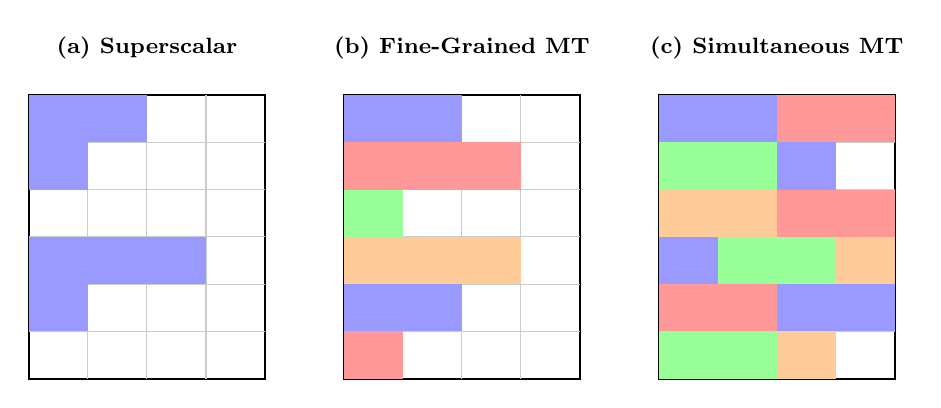
\begin{tikzpicture}[>=stealth, font=\small]
    % --- Superscalar (Issue Waste) ---
    \node [font=\bfseries\footnotesize] at (1.5, 4.2) {(a) Superscalar};
    \draw [thick] (0,0) rectangle (3,3.6);
    % Grid lines (4-wide, 6 cycles)
    \foreach \y in {0.6, 1.2, 1.8, 2.4, 3.0} \draw [gray!40] (0,\y) -- (3,\y);
    \foreach \x in {0.75, 1.5, 2.25} \draw [gray!40] (\x,0) -- (\x,3.6);
    % Filled slots (Thread 1)
    \fill [blue!40] (0,3.0) rectangle (1.5,3.6); % Cycle 1: 2 insts
    \fill [blue!40] (0,2.4) rectangle (0.75,3.0); % Cycle 2: 1 inst (Horiz)
    % Cycle 3: Vertical waste
    \fill [blue!40] (0,1.2) rectangle (2.25,1.8); % Cycle 4: 3 insts
    \fill [blue!40] (0,0.6) rectangle (0.75,1.2); % Cycle 5: 1 inst
    
    % --- Fine-Grained Multithreading ---
    \node [font=\bfseries\footnotesize] at (5.5, 4.2) {(b) Fine-Grained MT};
    \draw [thick] (4,0) rectangle (7,3.6);
    \foreach \y in {0.6, 1.2, 1.8, 2.4, 3.0} \draw [gray!40] (4,\y) -- (7,\y);
    \foreach \x in {4.75, 5.5, 6.25} \draw [gray!40] (\x,0) -- (\x,3.6);
    % Interleaved threads per cycle
    \fill [blue!40] (4,3.0) rectangle (5.5,3.6);   % T1
    \fill [red!40]  (4,2.4) rectangle (6.25,3.0);  % T2
    \fill [green!40](4,1.8) rectangle (4.75,2.4);  % T3
    \fill [orange!40](4,1.2) rectangle (6.25,1.8); % T4
    \fill [blue!40] (4,0.6) rectangle (5.5,1.2);   % T1
    \fill [red!40]  (4,0.0) rectangle (4.75,0.6);  % T2

    % --- Simultaneous Multithreading (SMT) ---
    \node [font=\bfseries\footnotesize] at (9.5, 4.2) {(c) Simultaneous MT};
    \draw [thick] (8,0) rectangle (11,3.6);
    \foreach \y in {0.6, 1.2, 1.8, 2.4, 3.0} \draw [gray!40] (8,\y) -- (11,\y);
    \foreach \x in {8.75, 9.5, 10.25} \draw [gray!40] (\x,0) -- (\x,3.6);
    % Mixed threads within same cycle
    \fill [blue!40] (8,3.0) rectangle (9.5,3.6); \fill [red!40] (9.5,3.0) rectangle (11,3.6);
    \fill [green!40] (8,2.4) rectangle (9.5,2.4+0.6); \fill [blue!40] (9.5,2.4) rectangle (10.25,2.4+0.6);
    \fill [orange!40] (8,1.8) rectangle (9.5,2.4); \fill [red!40] (9.5,1.8) rectangle (11,2.4);
    \fill [blue!40] (8,1.2) rectangle (8.75,1.8); \fill [green!40] (8.75,1.2) rectangle (10.25,1.8); \fill [orange!40] (10.25,1.2) rectangle (11,1.8);
    \fill [red!40] (8,0.6) rectangle (9.5,1.2); \fill [blue!40] (9.5,0.6) rectangle (11,1.2);
    \fill [green!40] (8,0.0) rectangle (9.5,0.6); \fill [orange!40] (9.5,0.0) rectangle (10.25,0.6);
\end{tikzpicture}
\caption{Comparison of pipeline issue slot utilization across execution paradigms: white space represents combined vertical and horizontal waste.}
\label{fig:smt_pipeline_waste}
\end{figure}

\section{Simultaneous Multithreading (\glsfmtshort{smt})}
\label{sec:smt}

\glsxtrfull{smt} leverages the hardware infrastructure of a dynamically scheduled out-of-order superscalar processor to issue instructions from multiple independent threads within the same clock cycle.

\begin{concept}{Hardware Primitives for \glsfmtshort{smt}}{smt-primitives}
    A dynamic out-of-order superscalar core natively provides key primitives required for \gls{smt}:
    \begin{enumerate}
        \item \textbf{Unified \glsxtrfull{prf}:} Holds active, committed, and speculative state across multiple threads.
        \item \textbf{\glsxtrfullpl{rat}:} Duplicated per thread to rename architectural register names ($R_0 \dots R_n$) to the shared physical register pool dynamically.
        \item \textbf{Out-of-Order Instruction Queues and \gls{cdb}:} Instruction windows, reservation stations, and \glsxtrfull{cdb} snoop tags across threads seamlessly without structural partition barriers.
    \end{enumerate}
\end{concept}

By renaming thread-local architectural registers to shared physical registers, instructions from distinct threads flow through issue queues and functional units without requiring static hardware partitioning.

\subsection{\glsfmtshort{smt} Architectural Trade-offs and Evaluation}

Microarchitectural evaluations on multi-issue baselines (such as an 8-issue superscalar engine with 10 functional units) highlight the trade-offs between scheduling complexity and throughput:

\begin{itemize}
    \item \textbf{Single-Issue \gls{smt} / Fine-Grained Issue:} Restricts the fetch and decode stage to a single thread per cycle, but permits dynamic execution across multiple threads downstream.
    \item \textbf{Full-Issue \gls{smt}:} Allows instructions from multiple threads to be fetched, decoded, and issued simultaneously within the same clock cycle, completely filling issue bandwidth at the cost of complex fetch-prioritization logic (e.g., \textsf{ICOUNT} schemes favoring threads with fewest in-flight instructions).
\end{itemize}

\section{Multiprocessing vs. Hardware Multithreading}
\label{sec:multiprocessing_vs_multithreading}

Both \glsxtrfull{cmp} and \gls{smt} exploit \gls{tlp}, but they partition hardware execution resources differently.

\begin{table}[htbp]
\centering
\caption{Architectural Comparison: Multiprocessing vs. Hardware Multithreading}
\label{tab:cmp_vs_smt}
\small
\setlength{\tabcolsep}{6pt}
\begin{tabularx}{\textwidth}{|>{\hsize=0.8\hsize\raggedright\arraybackslash}X|>{\hsize=1.1\hsize\raggedright\arraybackslash}X|>{\hsize=1.1\hsize\raggedright\arraybackslash}X|}
\hline
\textbf{Dimension} & \textbf{Multiprocessing (\gls{cmp} / Multi-Core)} & \textbf{Multithreading (\gls{smt})} \\ \hline
\textbf{Resource Partitioning} & \textbf{Static Partitioning:} Each core has dedicated execution pipelines, functional units, and L1 caches. & \textbf{Dynamic Partitioning:} Execution units, caches, and buses are shared dynamically cycle-by-cycle. \\ \hline
\textbf{Hardware Overhead} & High area overhead (duplication of complete superscalar core logic). & Low area overhead ($\sim 5\text{--}10\%$ addition for duplicated \glspl{pc}, \glspl{rat}, and architectural registers). \\ \hline
\textbf{Single-Thread Performance} & Maximum performance per core (no inter-thread resource contention). & Slightly degraded due to shared L1 cache footprint and queue contention. \\ \hline
\textbf{Inter-Thread Interference} & Low (sharing occurs primarily at L2/L3 cache levels). & High (threads compete for execution slots, caches, and branch predictors). \\ \hline
\end{tabularx}
\end{table}

\begin{concept}{Core Resource Partitioning Principle}{resource-partitioning-principle}
    \begin{itemize}
        \item \textbf{Multiprocessors} allocate physical execution resources \textbf{statically} to independent threads (separate physical cores).
        \item \textbf{Multithreaded Processors} allocate physical execution resources \textbf{dynamically} on a cycle-by-cycle basis across shared functional units.
    \end{itemize}
\end{concept}

\section{Design Challenges in \glsfmtshort{smt}}
\label{sec:smt_design_challenges}

While \glsxtrfull{smt} maximizes hardware slot utilization by interleaving instructions from multiple threads, integrating \gls{smt} into high-performance out-of-order engines introduces critical microarchitectural trade-offs across single-thread performance, critical-path timing, and memory hierarchy access.

\subsection{Single-Thread Performance vs. System Throughput}

Because \gls{smt} relies on fine-grained dynamic scheduling across shared functional units, inter-thread resource competition directly impacts single-thread completion latency:
\begin{itemize}
    \item \textbf{Preferred Thread Scheduling:} To mitigate single-thread latency degradation, microarchitectures may employ a \textit{preferred thread} policy, prioritizing issue slots for a primary thread. However, if the preferred thread stalls on a high-latency event (e.g., an L2/L3 cache miss), pipeline throughput drops significantly because secondary threads were denied early entry into issue queues.
    \item \textbf{Throughput Optimization:} Overall system throughput is maximized only when a sufficient pool of active, independent threads is available to fill empty issue slots dynamically and hide long-latency memory stalls completely.
\end{itemize}

\subsection{Hardware Complexity and Critical Paths}

Scaling a dynamic superscalar core to support multi-thread execution expands several critical execution structures:
\begin{itemize}
    \item \textbf{Register File Footprint and Access Latency:} Supporting $T$ hardware threads requires expanding the unified \glsxtrfull{prf} to hold $T$ complete architectural register sets alongside speculative in-flight outputs. The increased register array size and multiporting requirements lengthen read/write access paths, potentially impacting clock frequency.
    \item \textbf{Instruction Fetch Bandwidth:} Front-end engines must fetch high-bandwidth instruction streams across non-contiguous memory spaces for multiple threads simultaneously, placing severe strain on L1 Instruction Cache ($I$-cache) read ports and branch predictor entry capacity.
    \item \textbf{Issue Logic and Clock Cycle Time:} Multi-thread register renaming, intra-cycle hazard detection comparators, and dynamic instruction queue prioritization (e.g., \textsf{ICOUNT} schemes) increase gate complexity on the critical pipeline path.
\end{itemize}

\subsection{Memory Hierarchy Contention}

Executing multiple instruction streams concurrently on a single physical core amplifies interference across the memory hierarchy:
\begin{itemize}
    \item \textbf{Cache Thrashing:} Independent thread working sets compete directly for finite L1 data and instruction cache lines, leading to mutual cache line evictions and degraded individual thread execution times.
    \item \textbf{\gls{tlb} Conflicts:} Concurrent address space traversals increase pressure on shared \glsxtrfull{tlb}, requiring tag filtering via \glsxtrfull{asid} to prevent frequent translation misses.
\end{itemize}

\section{Empirical Comparison of Real-World \glsfmtshort{ilp} Microarchitectures}
\label{sec:empirical_ilp_microarchitectures}

The theoretical limits of \glsxtrfull{ilp} manifest differently across commercial microarchitectural paradigms. Historical evaluations across diverse hardware designs—such as the AMD Athlon, Intel Pentium 4, Intel Itanium 2, and IBM POWER5—demonstrate that no single architecture dominates across all performance and efficiency metrics.

\begin{observation}{Microarchitectural Performance and Area Efficiency}{ilp-real-world-comparison}
Comparative evaluations using standard SPEC CPU benchmarks reveal distinct trade-offs between dynamic dynamic issue complexity, static compiler scheduling, and energy consumption:
\begin{itemize}
    \item \textbf{Integer Throughput (SPECint):} The out-of-order AMD Athlon leads in SPECint performance, followed by the Intel Pentium 4, Intel Itanium 2, and IBM POWER5.
    \item \textbf{Floating-Point Throughput (SPECFP):} The IBM POWER5 and Intel Itanium 2 dominate floating-point workloads, outperforming the Athlon and Pentium 4 by a wide margin.
    \item \textbf{Area and Transistor Efficiency:} The AMD Athlon and Intel Pentium 4 achieve high efficiency in terms of performance extracted per unit silicon area and transistor count.
    \item \textbf{Energy Efficiency (SPECFP / Watt):} The IBM POWER5 is the most energy-effective processor on SPECFP workloads and ties for top efficiency on SPECint. Conversely, the explicitly parallel static \gls{vliw} Intel Itanium 2 proves to be the most inefficient processor per watt and per area unit across both integer and floating-point codes (with the sole exception of floating-point throughput per watt).
\end{itemize}
\end{observation}

\begin{table}[htbp]
\centering
\caption{Empirical Trade-off Matrix of Commercial \gls{ilp} Microarchitectures}
\label{tab:real_world_ilp_processors}
\small
\setlength{\tabcolsep}{5pt}
\begin{tabularx}{\textwidth}{|>{\hsize=0.8\hsize\raggedright\arraybackslash}X|>{\hsize=1.0\hsize\raggedright\arraybackslash}X|>{\hsize=1.2\hsize\raggedright\arraybackslash}X|}
\hline
\textbf{Processor Architecture} & \textbf{Dominant Workload} & \textbf{Key Efficiency Profile} \\ \hline
\textbf{AMD Athlon} & SPECint Leader & High transistor and area efficiency \\ \hline
\textbf{Intel Pentium 4} & Balanced Integer & High clock frequency, good area utilization \\ \hline
\textbf{Intel Itanium 2 (\gls{vliw})} & SPECFP Co-Leader & Inefficient in area/power; bounded by slow clock rate \\ \hline
\textbf{IBM POWER5 (\gls{smt})} & SPECFP Co-Leader & Top overall energy efficiency (SPECFP / Watt) \\ \hline
\end{tabularx}
\end{table}

\section{Hardware and Energy Bounds to Wide-Issue Scaling}
\label{sec:hardware_energy_bounds_ilp}

Attempting to scale multi-issue superscalar processors beyond current limits (doubling issue rates from 3–6 instructions per cycle up to 6–12 instructions per cycle) encounters severe physical and microarchitectural walls.

\subsection{Front-End and Register File Scaling Bottlenecks}

To sustain a wide issue bandwidth of 6 to 12 instructions per clock cycle, the execution pipeline must simultaneously satisfy non-linear resource demands:

\begin{concept}{Resource Requirements for Wide Multi-Issue Scaling}{resource-wide-issue}
Sustaining an issue rate of $N = 6\text{--}12$ instructions per cycle requires hardware capable of:
\begin{enumerate}
    \item \textbf{Instruction Fetch Bandwidth:} Fetching 12 to 24 instructions per cycle from the L1 Instruction Cache across unpredictable branch boundaries.
    \item \textbf{Branch Resolution:} Resolving 2 to 3 conditional or unconditional branches per cycle.
    \item \textbf{Memory Access Multiporting:} Executing 3 to 4 simultaneous data memory accesses (loads/stores) per cycle.
    \item \textbf{Register File Porting:} Renaming and accessing more than 20 register ports per cycle in parallel.
\end{enumerate}
\end{concept}

The logic gate complexity required to perform intra-cycle dependency checks and rename logic scales quadratically ($\mathcal{O}(N^2)$). This combinatorial growth directly forces microarchitects to lower maximum clock frequencies. For example, the Intel Itanium 2 featured one of the widest issue rates of its era, yet suffered from the slowest maximum clock frequency despite consuming the highest overall power.

\subsection{The Energy Inefficiency of \glsfmtshort{ilp} Scaling}

Virtually all microarchitectural mechanisms designed to extract additional \gls{ilp} increase power consumption faster than they increase execution throughput.

\begin{definition}{The Peak vs. Sustained Performance Gap}{peak-sustained-gap}
Multiple-issue techniques exhibit inherent energy inefficiency due to two decoupled scaling functions:
\begin{align}
\text{Dynamic Transistors Switching} &\propto f(\text{Peak Issue Rate}) \\
\text{Realized Performance Gains} &\propto f(\text{Sustained Execution Rate})
\end{align}
Because the gap between peak issue capacity and sustained execution rate widens as issue width grows, wide superscalar engines expend an increasing amount of energy per unit of realized performance.
\end{definition}

\section{Empirical Performance and Energy Efficiency of \glsfmtshort{smt}}
\label{sec:empirical_smt_performance_energy}

To evaluate whether \glsxtrfull{smt} overcomes the energy inefficiency of \gls{ilp} scaling, Esmaeilzadeh et al. (2011) conducted an empirical evaluation on an Intel Core i7 processor (2-thread \gls{smt} core) using multithreaded workloads from the \textsf{PARSEC} parallel scientific suite and multithreaded Java applications.

\begin{observation}{Throughput Speedup under \glsfmtshort{smt}}{smt-speedup-results}
Enabling \gls{smt} on a single out-of-order core yields consistent throughput improvements across multithreaded workloads:
\begin{itemize}
    \item \textbf{Java Applications:} Achieves a harmonic mean performance speedup ratio of $1.28\times$. Removing two benchmarks constrained by limited intrinsic parallelism increases the harmonic mean speedup to $1.39\times$.
    \item \textbf{PARSEC Scientific Suite:} Achieves a harmonic mean performance speedup ratio of $1.31\times$.
\end{itemize}
\end{observation}

\subsection{Energy Efficiency Impact of \glsfmtshort{smt}}

Energy consumption is determined by the balance between execution speedup and the increased power draw resulting from active multithreaded hardware structures.

\begin{concept}{Energy Efficiency Ratio in \glsfmtshort{smt} Workloads}{smt-energy-efficiency}
    \begin{itemize}
        \item \textbf{Java Workloads:} Energy efficiency remains essentially neutral ($1.00\times$), as the power consumption increase matches the realized performance speedup.
        \item \textbf{PARSEC Workloads:} Achieves a net energy efficiency improvement ratio of $1.08\times$. 
    \end{itemize}
    This demonstrates a key microarchitectural insight: when \gls{smt} enables performance gains that outpace additional dynamic switching power, performance improvements directly translate into overall system energy efficiency.
\end{concept}

\section{Summary: The Limits of \glsfmtshort{ilp} and the Transition to Explicit Parallelism}
\label{sec:ilp_summary_shift_to_tlp}

Decades of microarchitectural research establish that practical limits—including the power wall, compiler limits, dependency chains, and quadratic logic complexity—cap dynamic superscalar issue widths at \textbf{3 to 6 instructions per cycle}.

\begin{concept}{Core Takeaways on Architectural Concurrency}{architectural-concurrency-takeaways}
    \begin{enumerate}
        \item \textbf{Ceiling of Implicit Concurrency:} Scaling dynamic \gls{ilp} hardware yields diminishing returns at unsustainable energy costs.
        \item \textbf{Shift to Explicit Parallelism:} High-performance computing relies on explicit software parallelism, primarily \textbf{\glsxtrfull{dlp}} and \textbf{\glsxtrfull{tlp}}.
        \item \textbf{Multithreading Paradigm Choice:} 
        \begin{itemize}
            \item \textit{Coarse-Grained Multithreading:} Context-switches only on high-latency memory stalls to avoid single-thread degradation.
            \item \textit{Fine-Grained Multithreading:} Interleaves threads cycle-by-cycle to hide short and long pipeline stalls.
            \item \textit{\glsxtrfull{smt}:} Integrates fine-grained multithreading into out-of-order superscalar architectures, dynamically reusing physical register renaming structures instead of statically duplicating full execution logic.
        \end{itemize}
    \end{enumerate}
\end{concept}